\section{Appendix: Sequence To Sequence Model} \label{sec:Seq2Seq}

\subsection{Describing Seq-to-Seq Model}


A \textbf{sequence-to-sequence (Seq-to-Seq) model} processes a sequence of embeddings. An \textbf{Encoder} squashes the source sequence $\overrightarrow{x} = \{ x_1, ..., x_{T_x} \}$ of individual word vectors $x_t$ in the input sentence $X$ into a \emph{fixed-length} \textbf{context vector} that is sent to a \textbf{Decoder} which outputs a target sequence one word at a time (Alammar, 2018a). 

Formally, an Encoder \hyperref[sec:GRU]{gated recurrent unit (GRU)} outputs a hidden state given a previous hidden state and the current input $h_t = \texttt{EncoderGRU} \Big( x_t, h_{t-1} \Big)$, where the context vector named $z$ is assigned the last hidden state: $z = h_{T_x}$. The context vector is then passed to the Decoder along with a target token $y_t$ and previous Decoder hidden state $s_{t-1}$ to return a current hidden state, $s_t = \texttt{DecoderGRU} \Big( y_t, s_{t-1}, z \Big)$. The context vector $z$ does not have a time step $t$ subscript, signifying the same context vector from the Encoder is reused each time step in the Decoder. 




% \begin{figure}[h]
% \vspace{-5pt}
% \centering
% 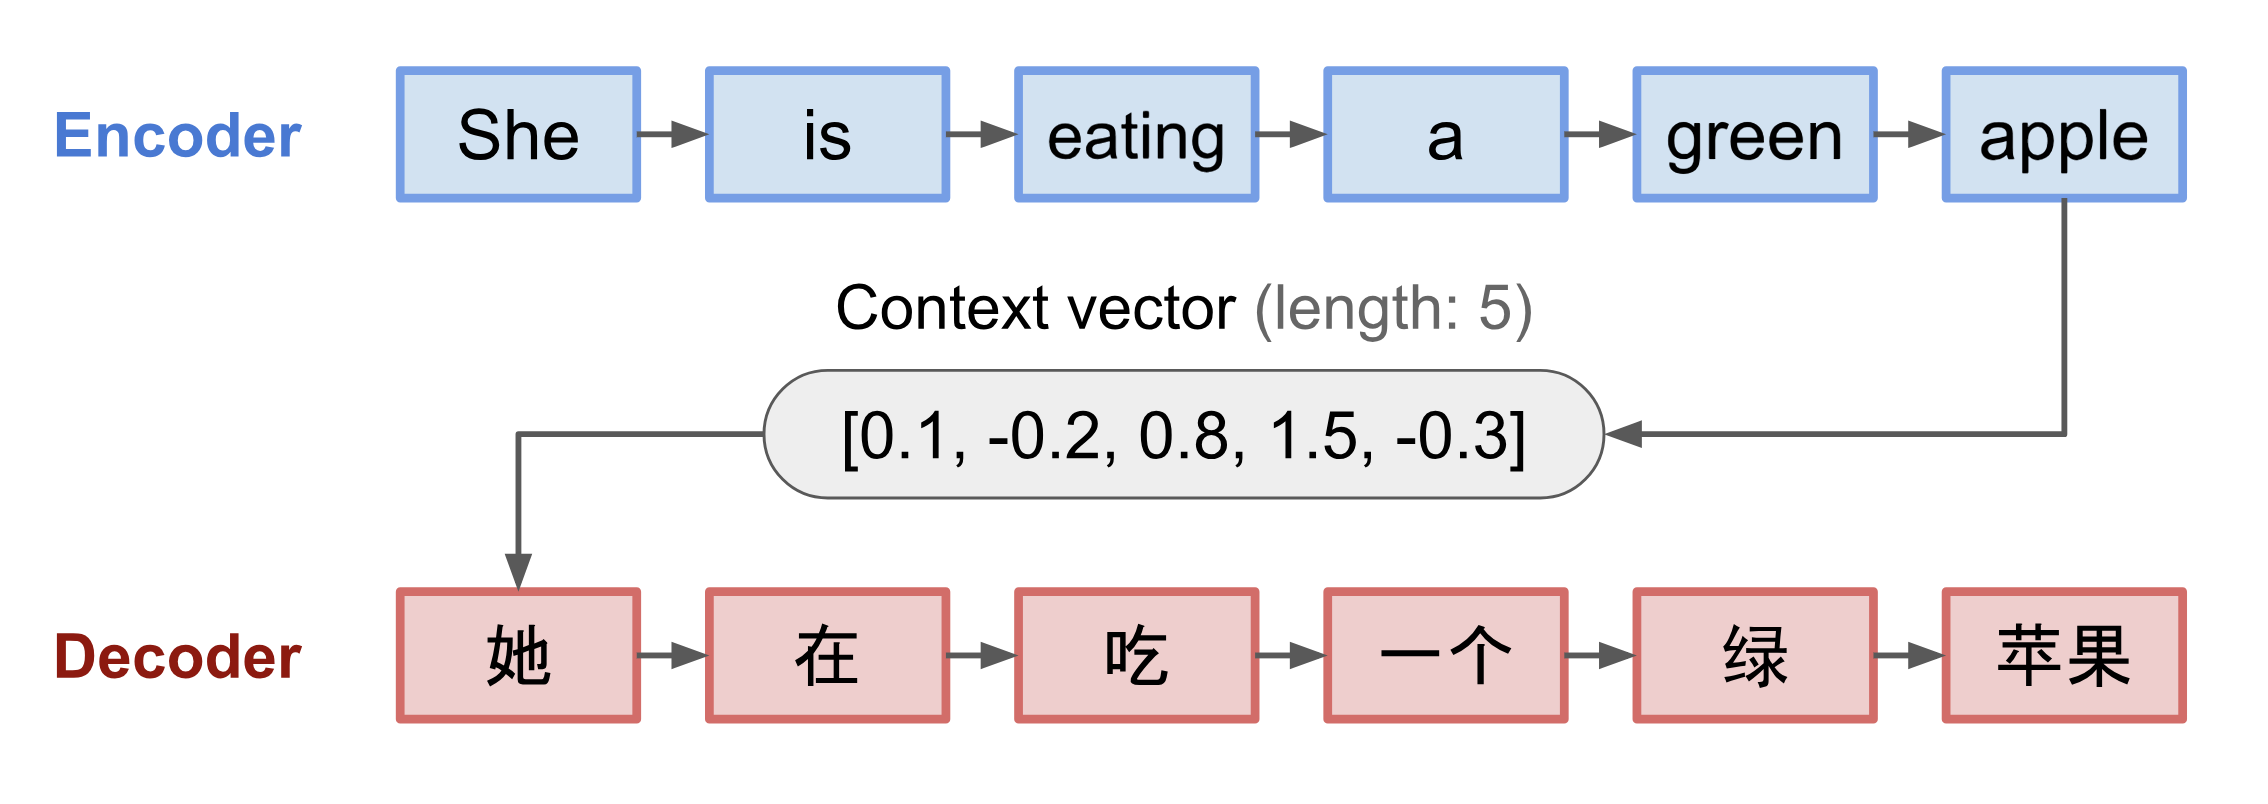
\includegraphics[width=0.6\textwidth]{imgs/seqtoseq_greenapple.png}
% \vspace{-5pt}
% \caption{\footnotesize Encoder-Decoder with Context Vector in a Seq-to-Seq model, translating the sentence ``She is eating a green apple" to Chinese. From \emph{Attention? Attention!}, by Weng, 2018. \url{https://lilianweng.github.io/lil-log/2018/06/24/attention-attention.html}. Copyright 2018 by Weng.}
% \vspace{-5pt}
% \end{figure}


\subsection{Problem with Seq-to-Seq Models} \label{sec:ProblemWithSeq2Seq}

The context vector $z$ does not have a time step $t$ subscript, meaning this same context vector from the Encoder is reused each time step in the Decoder. Essentially, compressing the inputs into such a \textbf{fixed-length} vector leads to a \textbf{long-term dependency problem} since the Decoder uses only the last hidden state of the Encoder, not all hidden states. 


\subsection{The Attention Mechanism} \label{sec:AttentionMechanism}


{
\begin{wrapfigure}{L}{0.5\textwidth}
\begin{center}
    \vspace{-20pt}
    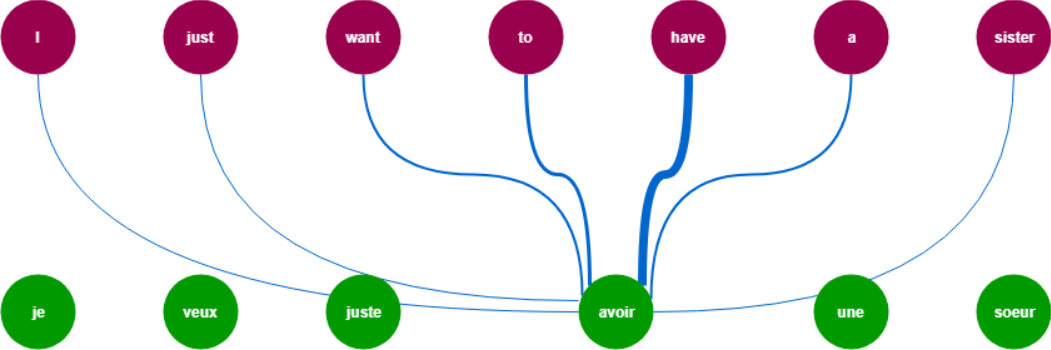
\includegraphics[width=\linewidth]{imgs/attention.png}
\end{center}
\vspace{-10pt}
\captionof{figure}{Attention Mechanism: How words are considered for contextual evidence. From \emph{Intuitive Understanding of Seq2seq model and Attention Mechanism in Deep Learning}, by Medium, 2019. \href{https://medium.com/analytics-vidhya/intuitive-understanding-of-seq2seq-model-attention-mechanism-in-deep-learning-1c1c24aace1e}{https://medium.com/analytics-vidhya}. Copyright n.d by n.d.}
%\vspace{15pt}
\label{fig:attention}
\end{wrapfigure}

The \textbf{attention mechanism} was proposed in \nameref{nlptask:neuralmachinetranslationNMT} task to memorize longer sentences by ``selectively focusing on parts of the source sentence" as required (Luong et al., 2015). Instead of creating a single context vector $z$ from the Encoder's last hidden state $h_{T_x}$, the \emph{attention architecture} creates a context vector for each input word or timestep $t$, reducing the information compression problem by letting the Decoder use all Encoder hidden states. The attention mechanism essentially creates links between the context vector and entire source input. A general illustration is in \cref{fig:attention}.

\subsection{Seq-to-Seq Model Using Attention}

The key components of a Seq-to-Seq model with attention are its Attention forward pass, which computes attention scores, and Decoder forward pass, which outputs the context vector. 

}


\subsubsection{Forward Pass of Attention}

The attention mechanism is viewed as a layer in the Seq-to-Seq model with a forward pass that updates parameters. The steps for the forward pass to calculate attention scores $\alpha_{ti}$ is as follows: 

\begin{enumerateSpaced}{3pt}
    \item First, an \textbf{alignment model} \texttt{align} calculates \textbf{energy scores} $e_{ti}$ that measure how well the ``inputs around position $i$ and the output at position $t$ match" (Bahdanau et al., 2016). The energy scores $e_{ti} = \texttt{align} \Big(s_{t-1}, h_i \Big)$ are weights specifying how much of the Decoder hidden state $s_{t-1}$ and the Encoder hidden state $h_i$ of the source sentence should be considered for each output (Ta-Chun, 2018; Bahdanau et al., 2016). 
    
    \item Next, the energy score $e_{ti}$ is passed through a \hyperref[sec:NeuralLM]{feed-forward neural network} and \hyperref[cnc:softmaxLayer]{softmax} to calculate the attention scores in \cref{eq:AlignScores}, ensuring the attention vector $\overrightarrow{\alpha} = \Big \{ \alpha_{ti} \Big \}$ has values normalized between $0$ and $1$:
    \begin{equation}
    \alpha_{ti} = \frac{\exp{(e_{ti})} } { \sum_{k=1}^{T_x} \exp{(e_{ik})} } 
    \label{eq:AlignScores}
    \end{equation}
\end{enumerateSpaced}


\subsubsection{Forward Pass of Decoder}

Once the attention scores have been calculated, the Decoder calculates the context vector, $c_t = \sum_{i=1}^{T_x} \alpha_{ti} \cdot h_i$, which is a sum of Encoder hidden states $h_i$ weighted by attention scores $\overrightarrow{\alpha} = \Big \{ \alpha_{ti} \Big \}$ (Ta-Chun, 2018). Intuitively, the context vector is an \textbf{expectation}. 

%The attention score $\alpha_{ti}$ is the probability that target word $y_t$ is aligned to (or translated from) an input word $x_j$. Then $c_t$ is the expected hidden state over all hidden states $h_i$ with probabilities $\alpha_{ti}$, which quantify the importance of Encoder hidden state $h_i$ with respect to the previous Decoder hidden state $s_{t-1}$ in deciding the next Decoder state $s_t$ for generating target word $y_t$.   

Through this attention mechanism, the Seq-To-Seq model relieves the Encoder from having to compress all source sentence information into a fixed-length vector, allowing the information to spread through the hidden state sequence $\overrightarrow{h} = \Big \{ h_1,...,h_T\Big \}$ and later be detected by the Decoder (Trevett, 2020).  


%\subsubsection{Forward Pass of Seq-to-Seq Model}
%
%Finally, the Seq-to-Seq model can use the Encoder, Decoder and attention in conjunction. Its \hyperref[sec:ForwardProp]{forward pass} is (Trevett, 2020): 

% \begin{enumerateSpaced}{3pt}
%     \item Create an output tensor to hold predicted words $\hat{y}$
%     
%     \item Pass the source sequence $\overrightarrow{x} = \Big \{ x_1, ..., x_T \Big \}$ into the Encoder to receive the contexts $\overrightarrow{z}$ alongside the hidden states $\overrightarrow{h} = \Big \{ h_1, ..., h_T \Big \}$.
%     
%     \item Set equal the initial Decoder hidden state $s_0$ and last Encoder hidden state $h_T$.
%     
%     \item Decode within a loop: insert the target token $y_t$ and previous hidden state $s_t$ and all Encoder outputs $\overrightarrow{h}$ into the Decoder to get a prediction $\hat{y}_{t+1}$ and new hidden state $s_t$.
%     
%     
% \end{enumerateSpaced}
